% ===================================================================
% Capítulo 7 — Considerações Finais
% ===================================================================
\chapter{CONSIDERAÇÕES FINAIS}
\label{cap:consideracoes}

\begin{figure}[H]
    \centering
    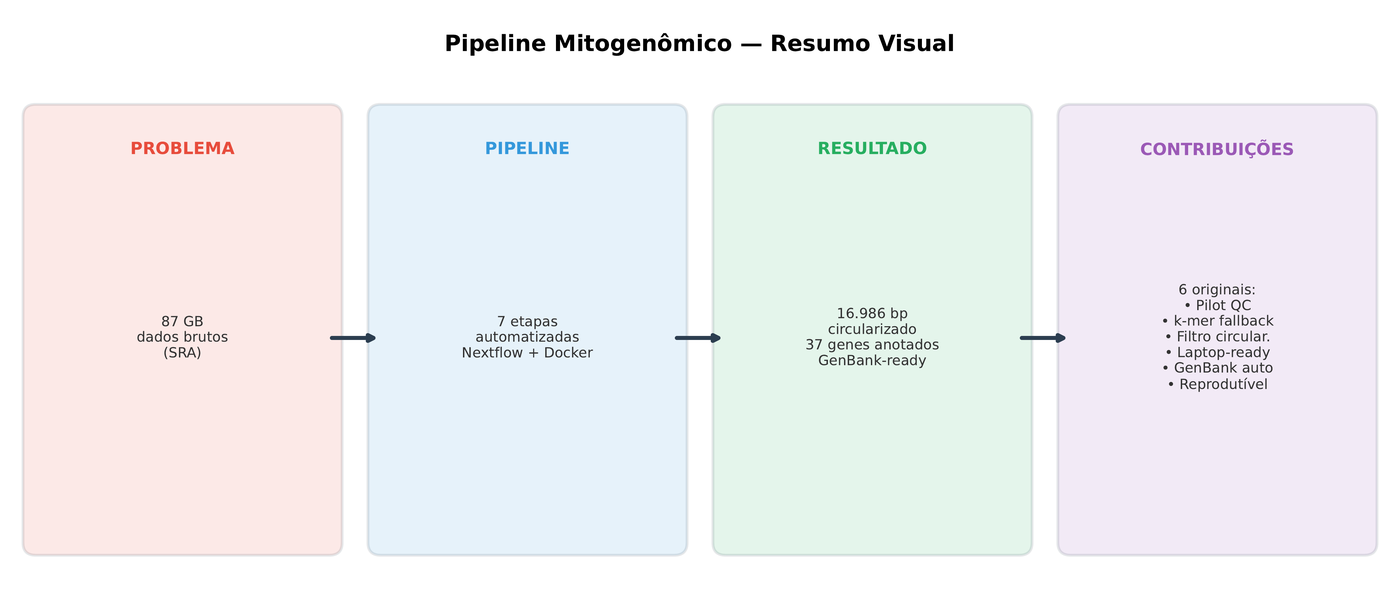
\includegraphics[width=\textwidth]{imagens/infografico_resumo.png}
    \caption{Infográfico-resumo do trabalho: do problema inicial (87~GB de dados brutos), passando pelas 7 etapas do pipeline, até o resultado final (16.986~bp circularizado, 37 genes, GenBank-ready) e as 6 contribuições originais.}
    \label{fig:infografico_resumo}
\end{figure}

O presente trabalho teve como objetivo propor e implementar um pipeline de bioinformática voltado à montagem e anotação funcional de genomas mitocondriais, concebido segundo princípios de automação, reprodutibilidade, ciência aberta e acessibilidade computacional. A integração de sete ferramentas consolidadas --- SRA-Toolkit, FastQC, Trim Galore com Cutadapt, NOVOPlasty, MITOS2, ViennaRNA e Biopython \cite{cock2009} --- em um fluxo containerizado (Docker) e orquestrado por meio do Nextflow constitui a principal contribuição metodológica desta proposta, ao oferecer uma solução transparente, portável e replicável para análises genômicas.

Um resultado particularmente significativo deste trabalho é a demonstração de que a montagem e anotação completa de mitogenomas a partir de dados públicos é viável em hardware doméstico. O dataset original utilizado totaliza 87\,GB de leituras brutas --- volume que, sem as estratégias de redução implementadas, exigiria centenas de gigabytes de armazenamento temporário e servidores dedicados. A cadeia de reduções progressivas incorporada ao pipeline (Pilot QC, truncamento adaptativo, \textit{trimming}) reduz esse volume em aproximadamente 5 milhões de vezes, viabilizando a execução em notebooks com 16\,GB de RAM em menos de uma hora. Essa acessibilidade é especialmente relevante para estudantes, pesquisadores iniciantes e instituições com recursos computacionais limitados, que anteriormente dependeriam de acesso a servidores ou \textit{clusters} para realizar análises genômicas equivalentes.

Do ponto de vista biológico, o pipeline foi aplicado com sucesso à montagem do mitogenoma da arara-azul-de-lear (16.986\,bp circularizado, 306$\times$ de cobertura, 37 genes identificados) e à espécie de validação \textit{Diploprion bifasciatus} (circularizado). Conforme detalhado no Capítulo~\ref{cap:mitogenoma}, a caracterização completa do mitogenoma da arara-azul-de-lear revelou composição nucleotídica, organização gênica e assinaturas moleculares (como o \textit{frameshift} do ND3) consistentes com a espécie congênere \textit{A. hyacinthinus}, confirmando a qualidade da montagem e a aplicabilidade dos dados para estudos de conservação, identificação forense e filogeografia.

Dentre as contribuições originais do pipeline, destacam-se:

\begin{enumerate}[label=(\roman*)]
    \item o módulo Pilot QC, que determina automaticamente o volume de dados necessário para atingir a cobertura desejada, evitando processamento desnecessário e viabilizando a execução em computadores com armazenamento limitado;
    \item a cadeia de reduções progressivas (Pilot QC $\rightarrow$ truncamento $\rightarrow$ \textit{trimming}) que transforma 87\,GB de dados brutos em um mitogenoma de 17\,KB, eliminando a necessidade de servidores dedicados;
    \item a lógica iterativa de montagem com \textit{re-seeding} automático e múltiplos \textit{k-mers};
    \item a geração automática de estruturas secundárias de tRNAs e rRNAs via RNAplot/ViennaRNA, funcionalidade anteriormente restrita à interface web do MITOS2;
    \item a conversão automática para GenBank Flat File com tratamento do \textit{frameshift} do ND3; e
    \item a compilação automática de 14 categorias de entregáveis em pasta organizada.
\end{enumerate}

Apesar de seu potencial, algumas limitações precisam ser reconhecidas. O sucesso da montagem depende da qualidade da \textit{seed} inicial e da profundidade de cobertura dos dados de sequenciamento. A anotação do MITOS2, embora automatizada, pode requerer curadoria manual em casos de estruturas gênicas atípicas (como o \textit{frameshift} do ND3). Adicionalmente, o tamanho dos \textit{containers} Docker ($\sim$2--4\,GB por imagem) pode representar uma barreira em ambientes com espaço de armazenamento limitado.

Como perspectivas futuras, propõem-se:

\begin{enumerate}[label=(\roman*)]
    \item a validação da montagem de \textit{D.~bifasciatus} por BLAST contra a referência PZ143763.1 do GenBank;
    \item a submissão do mitogenoma da arara-azul-de-lear ao GenBank;
    \item a integração de análises filogenéticas automáticas ao pipeline (MAFFT + RAxML/\allowbreak IQ-TREE);
    \item a geração automática de tabelas de RSCU (\textit{Relative Synonymous Codon Usage}) e de razão Ka/Ks para análise de pressão seletiva sobre os genes codificadores --- análises que se tornaram padrão em estudos recentes de genômica mitocondrial \cite{zhan2024,kundu2024,shi2024};
    \item a integração de tRNAscan-SE como módulo opcional de verificação dos tRNAs preditos pelo MITOS2, seguindo a prática consolidada na literatura;
    \item a geração de gráficos de sintenia comparativa entre espécies congêneres; e
    \item a publicação do pipeline no nf-core como recurso comunitário.
\end{enumerate}

Em síntese, o pipeline desenvolvido representa uma contribuição metodológica significativa para a bioinformática de organelas, ao unir rigor técnico, aplicabilidade biológica e boas práticas de reprodutibilidade computacional. Mais do que atender a um caso de estudo específico, constitui um recurso com potencial de ser reutilizado, adaptado e expandido por diferentes grupos de pesquisa, colaborando para a consolidação de uma ciência mais transparente, padronizada e sustentável.
